%Direct Quote: "widening of the spike shape, decrease of the firing rate and change in the interspike interval distribution". %All these single unit waveform shapes increased their width with temperature.\cite{goldin2017temperature}

\section{Which Limitations are Due to Abstract Models?}
\label{sec:optimization-performance}

Some of the limitations in the optimization of reduced models may come from their form; the abstractions they encode in their equations and parameters may come at the price of failing to exhibit key electrophysiological behaviors.

\subsection{A Somatosensory Layer 5 Pyramidal Neuron Model}
In order to test this, I extend the same optimization framework to a multi-compartmental, conductance based layer 5 pyramidal cell model \citep{van2016bluepyopt} (Figure \ref{fig:brief_shape}).
This model subserved as one of many component neurons in the original formulation of the Blue Brain Project \cite{markram2015reconstruction}.

\begin{figure}%{.2\textwidth}
  \begin{center}
    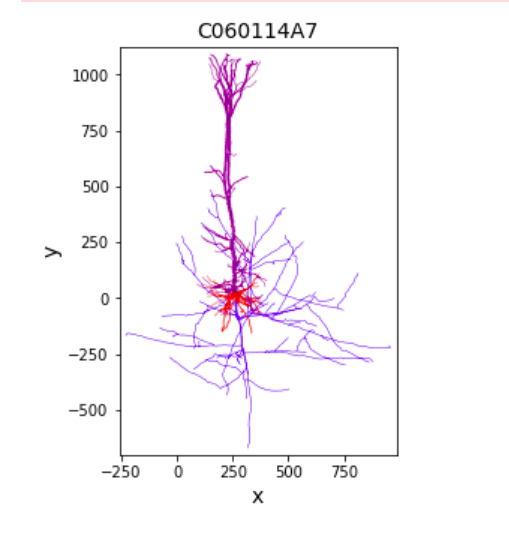
\includegraphics[scale=0.8]{figures/morphology_view.png}
    \caption[Visualization of a Reconstructed Layer 5 Pyramidal Neuron]{\textbf{Visualization of a Reconstructed Layer 5 Pyramidal Neuron}.
    Unlike the reduced model which has point geometry, the Layer 5 pyramidal neuron is spatially extended.
    Regions of the neuron with distinct sets of parameters are color coded: apical dendrites (magenta), basal dendrites (red), and axons (purple).
    }
  \label{fig:brief_shape}
  \end{center}
\end{figure}

This elaborate biophysical model is philosophically the opposite of the reduced models focused on in the majority of my thesis work. This elaborate model incorporates complex, biophysically detailed phenomena instead of excluding them in the hopes of capturing the key dynamics of membrane potential time series.
For example, this model is capable of a phenomenon the back-propagating action potential (BaP). BaPs can move travel in reverse direction, when they originate from distal dendrites and arrive at the soma where BaPs are free to sumate with incoming EPSPs (\url{https://github.com/BlueBrain/BluePyOpt/blob/master/examples/l5pc/L5PC.ipynb}).
This results in action potential waveforms far more complex than those produced by reduced models (none of which implement BaP waveforms at all) are capable of (Figs. \ref{fig:l5pc-a} and \ref{fig:l5pc-b}).

\begin{figure}
\centering
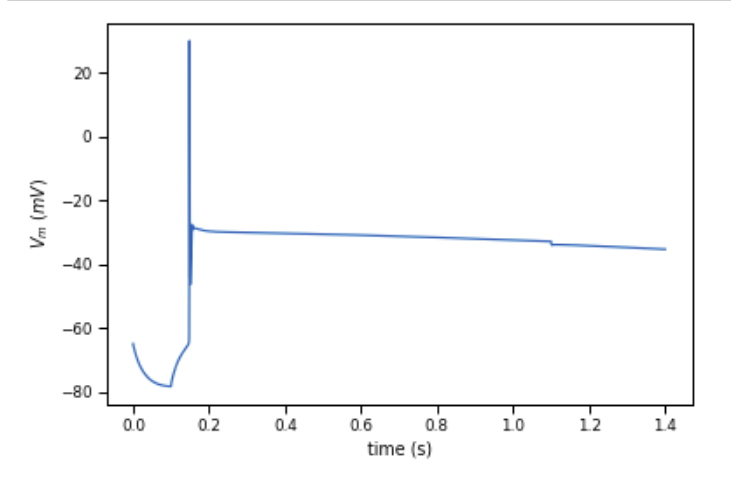
\includegraphics[scale=0.8]{figures/correct_active_l5pc.png}
\caption[AP Waveform in the L5PC model (A)]{\textbf{AP Waveform in the L5PC model}.
A current injection just sufficient for causing a single action potential (AP) is applied to the L5PC model soma, for one second from $100ms-1100ms$ in this model.
The AP waveform is briefer but more complex than reduced model AP shapes.
After the AP is complete, the somatic voltage plateaus at a depolarized level for the entire length of the simulation.
Genuine plateau potentials do occur in the L5PC dendrites, where $Ca^{2+}$ channels play a role \citep{zhu2000maturation}.
Plateau potentials in the dendrites typically result in a burst in the soma \emph{in vitro}. 
By contrast, a plateau potential in the soma is less common.
This phenomenon is driven by coupling to the distal dendrites, and are thus obviously neglected in reduced models of point neurons.}
\label{fig:l5pc-a}
\end{figure}

\begin{figure}
 \begin{center}
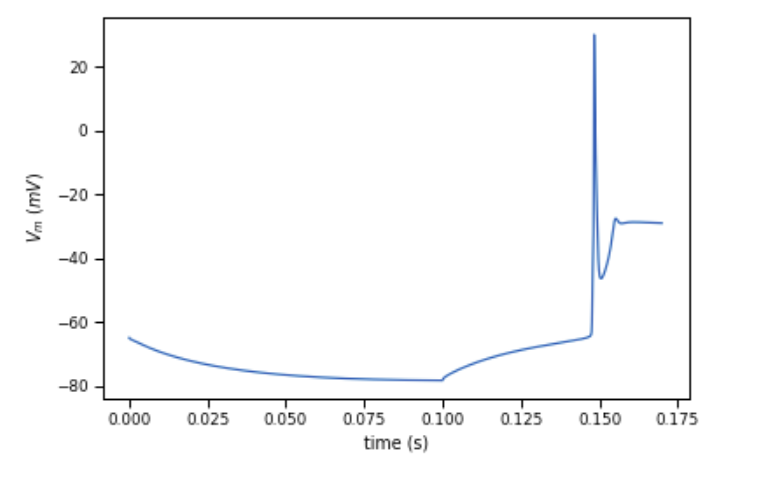
\includegraphics[scale=0.8]{figures/spike_shape.png}
\caption[AP Waveform in the L5PC model (B)]{\textbf{AP Waveform in the L5PC model}.
Same as Fig. \ref{fig:l5pc-a}, but zoomed into show spike onset and after hyperpolarization.}
\label{fig:l5pc-b}
\end{center}
\end{figure}

%\begin{figure}
%\begin{center}
%    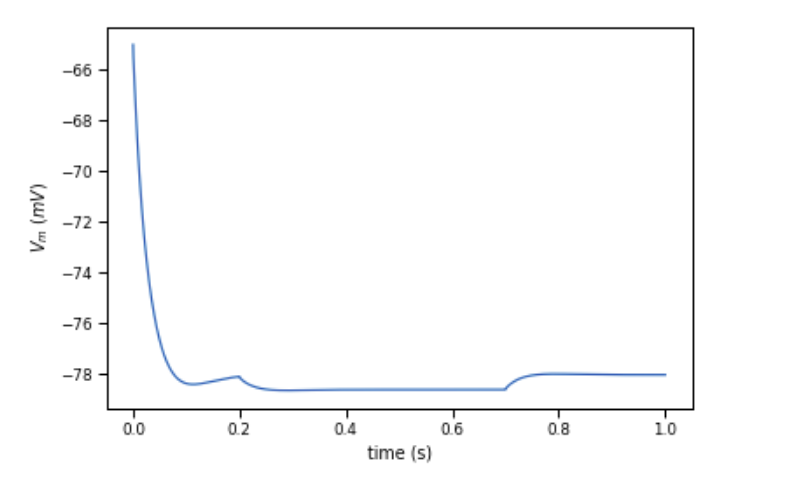
\includegraphics[scale=0.8]{figures/correct_passive_l5pc.png}
%    \caption[Subthreshold dynamics in the L5PC]{A current injection value of %-$10pA$ is applied to the soma of the pyramidal cell for the duration of %$200ms-700ms$. This plot shows the membrane potential at the soma of the %multi-compartment model displaying overall expected behavior, the trough of the %negative voltage deflection is not as deep as that seen in many reduced models. %This suggests the small amplitude of the negative deflection suggests that the L5 %PC model has less resistance than most of the reduced models fitted to the same %data, and indeed a low resistance measurement is confirmed in the table below.}
%  \label{fig:sub2}
%\end{center}
%\end{figure}

The model itself is extremely complex and contains many free parameters.
Some of these can be seen in the partial list of parameters in Figure \ref{fig:ca1_parameters}.
For example, these parameters include a number of distinct ionic conductances with distinct values in the soma, apical dendrites, and axon.
There are also other parameters (not displayed in Figure \ref{fig:ca1_parameters}) which are fixed, i.e. they are not modified during optimization.
\begin{center}
\begin{table}
\begin{tabular}{|l|r|}
\toprule
Parameter Name &           Value \\
\midrule
gNaTs2\_tbar\_NaTs2\_t.apical    &    0.0261 \\
gSKv3\_1bar\_SKv3\_1.apical      &    0.0042 \\
gImbar\_Im.apical              &    0.000143 \\
gNaTa\_tbar\_NaTa\_t.axonal      &    3.138 \\
gK\_Tstbar\_K\_Tst.axonal        &    0.0893 \\
gamma\_CaDynamics\_E2.axonal    &    0.00291 \\
gNap\_Et2bar\_Nap\_Et2.axonal    &    0.00683 \\
gSK\_E2bar\_SK\_E2.axonal        &    0.00710 \\
gCa\_HVAbar\_Ca\_HVA.axonal      &    0.000990 \\
gK\_Pstbar\_K\_Pst.axonal        &    0.974 \\
gSKv3\_1bar\_SKv3\_1.axonal      &    1.022 \\
decay\_CaDynamics\_E2.axonal    &  287.2 \\
gCa\_LVAstbar\_Ca\_LVAst.axonal  &    0.00875 \\
gamma\_CaDynamics\_E2.somatic   &    0.000609 \\
gSKv3\_1bar\_SKv3\_1.somatic     &    0.303 \\
gSK\_E2bar\_SK\_E2.somatic       &    0.00841 \\
gCa\_HVAbar\_Ca\_HVA.somatic     &    0.000994 \\
gNaTs2\_tbar\_NaTs2\_t.somatic   &    0.984 \\
decay\_CaDynamics\_E2.somatic   &  210.5 \\
gCa\_LVAstbar\_Ca\_LVAst.somatic &    0.000333 \\
\bottomrule
\end{tabular}

\caption[Subset of model parameters in the conductance-based L5PC neuron]{The Layer 5 Pyramidal Cell model (L5PC, \citep{van2016bluepyopt}
) contains hundreds of parameters, but only a subset of these are tunable.
A subset of 20, spanning conductances in the soma, apical dendrite, and axon, are shown here.
Most models considered in this thesis have $<14$ parameters; by contrast, having 20 parameters makes many approaches to model fitting intractable.
My optimizer explore the space spanned by these 20 parameters to produce a Primar Somatosensory Cortex Layer 5 Pyramdial Cell model that agrees with the experimental data.}
\label{fig:ca1_parameters}
\end{table}
\end{center}

%\begin{figure}
%    \begin{center}
%    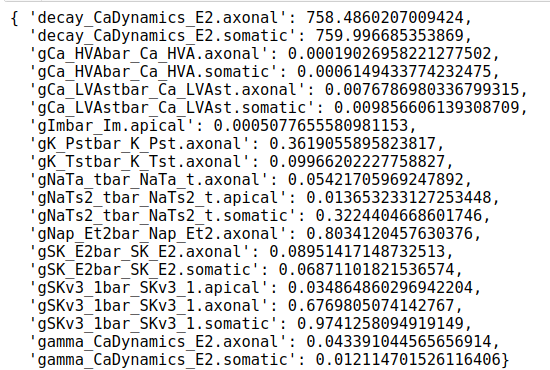
\includegraphics{figures/parameters_opt_l5pc.png}

%\end{figure}

An existing model of a layer 5 somato sensory rat, hind leg region was acquired by cloning an the BluePyOpt GitHub Repository \citep{van2016bluepyopt}.
In order to optimize this model using NeuronUnit tests, I created a dedicated NeuronUnit model simulation backend for this complex conductance-based, multi-compartmental model class.

I then applied my optimizer to this model and evaluated the quality of the resulting optimized model (Table \ref{table:l5pc-table}).
%Due to computational limitations this model was only run for 
%$\mu=12$ and $\NGEN=30$ generation. Actually a minimum of $\mu=100$, $NGEN %=100$ was prescribed by the scientists who optimized the initial model, however %such a large compute job required prohibitive computational resources.
The unoptimized model had statistics:\\
$(\chi^{2},p_{value})=(13.56, 0.094)$\\
Whereas the optimized model produced statistics:\\
$(\chi^{2},p_{value})$=$(6.63, 0.57)$.\\
Therefore, both the optimized and unoptimized model are not decisively outside the realm of biological plausibility according to the core NeuronUnit features, and optimization clearly improves such plausibility.
In both cases, this may in part reflect the highly variable nature of the biological/experimental results, rather than the verisimilitude of the optimized model.
Note that high variability of the values recorded for a given feature makes it very easy to achieve a Z-score of low magnitude (by the definition of a Z-score).

\begin{table}[ht]
\centering
\resizebox{\textwidth}{!}{
\begin{tabular}{|c|c|c|c|c|}%{lllll}
\toprule
Test Name & Observations & Predictions & Z-Scores & SEM \\
\midrule
RheobaseTest                   &    213.9 pA &      225.0 pA &  0.065 & 128.9 \\
InputResistanceTest            &  120.7 Mohm &  50.7 Mohm &  -0.90 & 27.9 \\
TimeConstantTest               &     15.7 ms &      16.76 ms &   0.14 & 2.6 \\
CapacitanceTest                &    150.6 pF &     330.7 pF &    1.28 & 1.49 \\
RestingPotentialTest           &    -68.3 mV &     -78.1 mV &   -1.5 & 44.0 \\
InjectedCurrentAPWidthTest     &      1.21 ms &       0.15 ms &   -1.98 & 0.175\\
InjectedCurrentAPAmplitudeTest &     80.4 mV &      89.6 mV &   0.72 & 1.49\\
InjectedCurrentAPThresholdTest &    -42.7 mV &     -59.6 mV &   -2.09 & 1.92\\
\bottomrule
\end{tabular}}
\caption[Observed and Predicted features for the Layer 5 Pyramidal Cell]{\textbf{Observed and Predicted features for the Layer 5 Pyramidal Cell}.
After equipping the L5PC model for NeuronUnit testing, this model was optimized against L5PC data from NeuroElectro.
Observed and predicted values could be made to agree on a subset of tests, such as rheobase and time constant, however in the larger test ensemble there was still a tradeoff in optimizing for one value vs another.
While this model falls within the range of biological plausibility ($\chi^2=13.6; p=0.094$),
the failure of the optimized model to achieve Z-scores consistently near zero suggests that, even with an extremely flexible conductance based model containing many parameters, the mean feature values reported in Neuroelectro are mostly likely mutually incompatible within a single neuron.}
\label{table:l5pc-table}
\end{table}

It is also worth noting that not optimized models vary depending upon which features are used to generated the constraining NeuronUnit test; one can improve optimization quality by choosing a subset of tests, as there was an irreconcilable trade-off between the membrane time constant, the action potential width, and the input resistance, with optimization only able to match the experimentally-reported means of only 1-2 (but not all 3) of these simultaneously.
Given this experimental variability and this trade-off between features, the optimization is at least satisfactory.
However, the inability of the optimizer to find an even better solution, with $Z=0$ across all features, indicated that there are fundamental conflicts between reported mean values across NeuroElectro features.
This conflict limits not only the possibility of optimizing reduced models, but also complex, multi-compartmental conductance-based models.
Therefore, reduced models do not appear to be the limiting concern; rather, data quality/consistency is.

\subsubsection{Caveats to the L5PC optimization}
It is also likely that many of the reported values in NeuroElectro were taken from experiments conducted at non-physiological temperatures.
Since temperature modulates action potential width \cite{goldin2017temperature} (and indeed all kinetic parameters), it is possible that a different result would be obtained if all data had been collected under the same, physiological temperature.

NeuroElectro lumps together layer 5 cortical pyramidal cells neurons from prefrontal cortex, somatosensory cortex, and primary visual cortex together into one dataset. 
Therefore it is also possible that while mean features across neurons of a single L5PC type (e.g. somatosensory) would have been mutually consistent, the frankenstein resulting from lumping all of these together was the source of the problems.

Finally, the L5PC model was very slow to simulate relative to the reduced models developed in this thesis work.
Where a single simulation of a typical reduced model described here is evaluated on average took only $~0.0025$ seconds, the L5PC model on average took $5.74$ seconds; evaluating the rheobase current required $34.8$ seconds.
Consequently it was difficult to run tens of thousands of simulations (across chromosomes and generations), especially in a development/debugging context.
The L5PC model documentation provide by the Blue Brain Project, suggests that $NGEN=100; \mu=100$ would define an appropriate GA search scale, however, due to time limitation I used smaller values. 
I nonetheless do not believe that longer optimization would have changed the major results, as the gains in fit quality would have been small.
However this unintentionally supports a major thrust of this thesis: if simulating very complex, very slow models doesn't solve any problems that simulating simple, fast ones does, then why bother with the former?


%%
% https://neuroelectro.org/data_table/36261/
%%
% from spike width table: 0.65 ± 0.13	1.04 ± 0.25**	0.51 ± 0.03**	0.59 ± 0.06	0.61 ± 0.03
%%
%

%\begin{figure}
%    \begin{center}
%    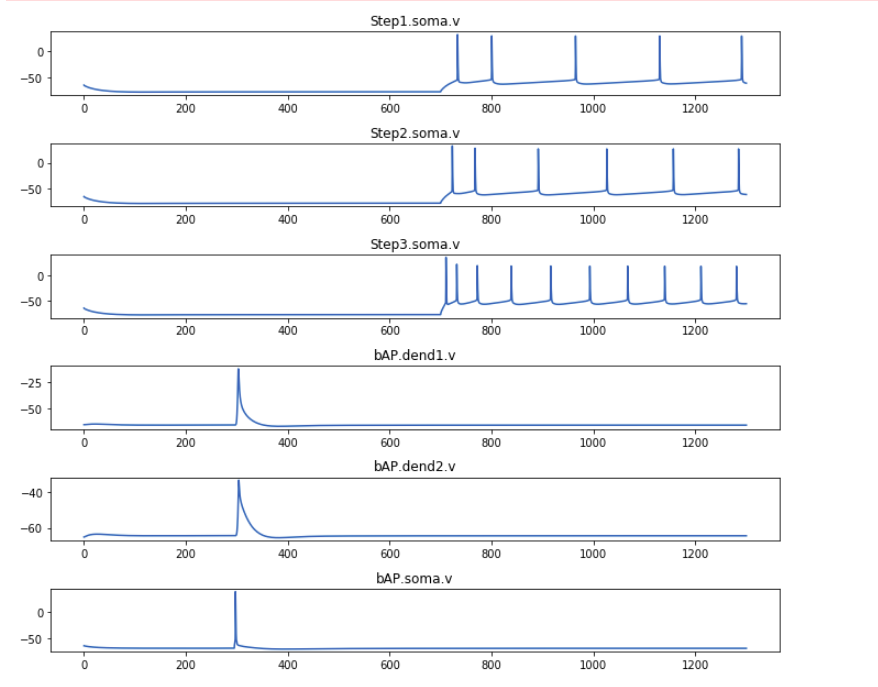
\includegraphics{figures/l5pc_before_opt}
    % \label{fig:my_label}
%    \end{center}
%\end{figure}


%Behavior of the L5PC model is explored under three different stimulus strengths.

%\begin{figure}
%    \begin{center}
%    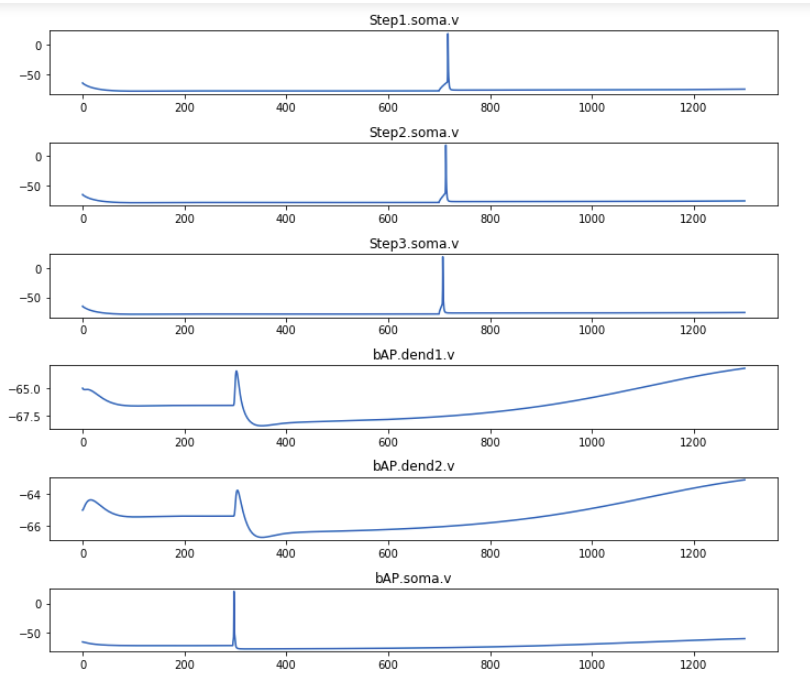
\includegraphics{figures/l5pc}
%    \caption[Behavior of the L5PC model under optimized parameters]{Behavior of %the L5PC model is explored under only one stimulus strength. Membrane potential %this time is viewed from recording locations in the soma and dendrites.  %Membrane potential this time is viewed from recording locations in the soma and %dendrites. In this recording site at the dendrite there is a singular %backpropogating spike. Although the soma and axon hillock, trigger an adapting %spike train, lasting more than a second, the dendrite only receives one %backpropogating potential, which has a large spike half width. The reason the %axon fires multiple times, but the dendrites fire once, is because  dendrites %contain dominating passive mechanisms, that can low pass filter invading %currents} 
%    \label{fig:after_optimization}
%    \end{center}
%\end{figure}    
    %\caption[Behavior of the L5PC model before optimization under default parameters]{}
%   }




%\begin{figure}
%\begin{center}
%   \includegraphics[scale=0.8]{figures/correct_a%ctive_l5pc.png}
%    \caption{A current injection sufficient for %causing a single spike is applied for a whole %second from $100ms-1100ms$}
%  \label{fig:sub1}
%  \end{center}
%\end{figure}

%As a reference point for understanding 
%    \caption{The spike shape is very brief in duration, and so it is worth zooming in for a closer look}

%\begin{figure}%{.2\textwidth}
%  \begin{center}
%    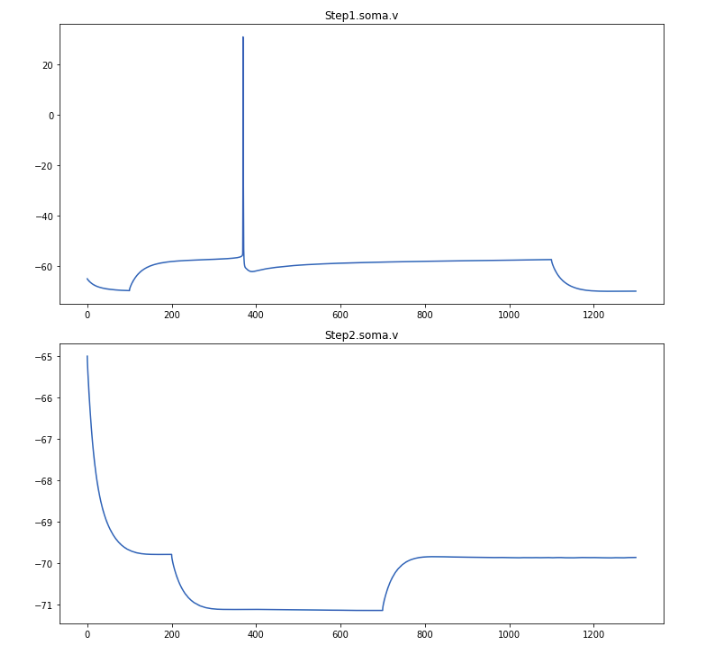
\includegraphics[scale=0.8]{figures/L5Somatosensory_not_optimized.png}
%    \caption[Plot of at threshold firing pyramidal neuron]{$V_{m}$ in $(mV)$ versus time $ms$, plots include a above threshold (top) and below threshold stimulus (below)}
%  \label{fig:brief_shape}
%  \end{center}
%\end{figure}

%\begin{figure}%{.2\textwidth}
%  \begin{center}
%    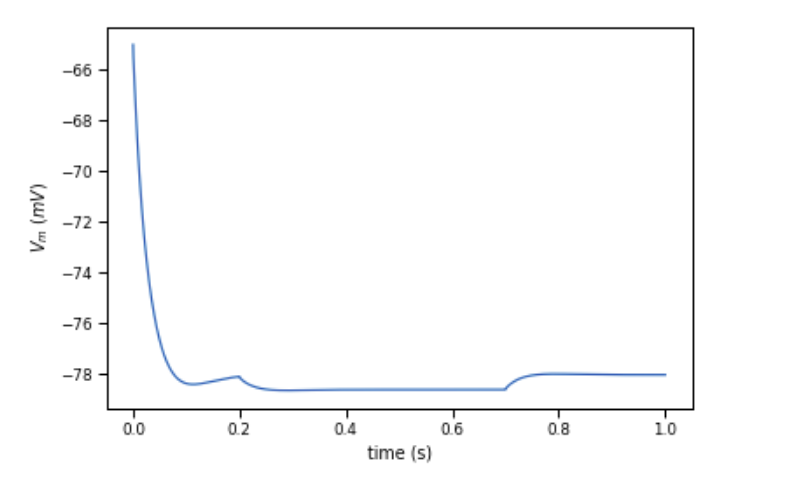
\includegraphics[scale=0.8]{figures/correct_passive_l5pc.png}
%    \caption[plot of negative amplitude current stimulus]{A current injection value of -$10pA$ is applied to the cell for the duration of $200ms-700ms$}
%  \label{fig:passive_properties}
%  \end{center}
%\end{figure}


